\section[Zuordnung der \acs{copra}-Biosignaldaten mit den \acs{fhir}-Profilen des Moduls \glqq Intensivmedizin\grqq{}]{Zuordnung der \acs{copra}-Biosignaldaten \\ mit den \acs{fhir}-Profilen des Moduls \glqq Intensivmedizin\grqq{}} \label{sect:resdatamapping}

Das Hauptziel dieser Arbeit wurde durch die ersten Schritten des Data Mappings der Biosignaldaten aus \ac{copra} mit den \ac{fhir}-Spezifikationen des Erweiterungsmoduls \glqq Intensivmedizin\grqq{} erreicht. Innerhalb dieser Schritte ist ein Datensatz mit der Zuordnung der \ac{copra}-Biosignaldaten mit den \ac{fhir}-Profilen entstanden. Mit Hilfe von diesem Datensatz wurden am Ende \ac{sql}-Views in die \ac{copra}-Instanz des Staging Bereichs des \ac{dw} des \ac{diz} programmiert. Solche virtuellen Tabellen dienen der Zusammenführung und Bereitstellung der Parameter beider Systeme und können somit das Gerüst für die \ac{fhir}-Ressourcen sein.

Am Ende dieses Projekts wurden 70 Biosignaldaten vom \ac{copra}-System richtig 39 \ac{fhir}-Profilen zugeordnet. Dieses Ergebnis wurde in einem Datensatz mit 75 Einträgen registriert.

Die meisten Werte der Bioparameter in \ac{copra} sind der Typ Dezimal (64), wie die \ref{fig:signaldatatyps} zeigt. Dieser Datentyp stimmt mit dem spezifizierten Datentyp des Attributs \texttt{val} des Elements \texttt{valueQuantity} in den \ac{fhir}-Profilen überein. Auch der Aufbau der Biosignaldaten für die Blutdruckmessungen in \ac{copra} stimmt mit der Struktur der \ac{fhir}-Profile überein. Nur eine Konfigurationsvariable war der Typ String (\ref{tab:stringvalue}) aber mit registrierten numerischen Werten, die bei der Programmierung der Transformationsregeln umgewandelt wurde (\ref{sec:prepdwtofhir}).

\begin{figure}[ht]
	\centering
	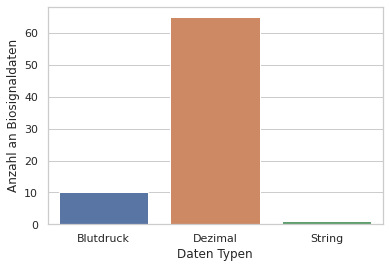
\includegraphics[height=8.5cm]{figures/biosignal_data_types}
	\caption[Datentypen der Biosignaldaten]{Datentypen der Biosignaldaten.}
	\label{fig:signaldatatyps}
\end{figure}

Auch die Distribution der Datenarten der \ac{fhir}-Profile ist zu berücksichtigen (\ref{fig:datenarten}). Die meist repräsentierte Datenart der Profile im Datensatz der Zuordnung ist die Art \glqq Parameter von Beatmung\grqq{} mit 36 zugeordneten Biosignaldaten. Diese Datenart ist auch die meist repräsentierte Art im Erweiterungsmodul \glqq Intensivmedizin\grqq{}.

\clearpage

\begin{figure}[ht]
	\centering
	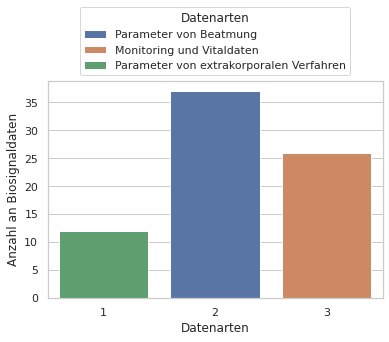
\includegraphics[height=8.5cm]{figures/datenarten}
	\caption[Datenarten der Profile]{Datenarten der Profile.}
	\label{fig:datenarten}
\end{figure}

